\chapter{Modelagem do Sistema e Projeto do Controlador LQG}\label{cap:ModelagemProjetoControlador}

Este capítulo abordará a descrição do modelo matemático do pêndulo invertido sobre duas rodas. Para a obtenção das equações do modelo, utilizará de Euler-Lagrange para tal fim. O eixo é fixo no centro das rodas, sendo assim, o mesmo só move quando há movimento linear das rodas. O ângulo de inclinação do pêndulo é o $\theta$, que é a variável controlada, e a velocidade angular é $\dot{\theta}$.

\section{Modelagem do Motor de Corrente Contínua}\label{sec:ModeloEletricoMotor}

O circuito elétrico simplificado que modele os motores CC do projeto, pode ser visto na Figura (\ref{fig:M-motor}) \citep{Silva:17}. 
\begin{figure}[H]
	\centering
	\includegraphics[scale=0.8]{Modelagem/Circuito_MotorDC.png}
	\caption{Representação esquemática do circuito elétrico do motor CC \citep{Silva:17}.}
	\label{fig:M-motor}
\end{figure}    

A variável $U$ representa a tensão de controle aplicada nos motores, $R$ e $L$ representam a resistência interna e a indutância dos enrolamentos do estator respectivamente. Aplicando a Lei das Tensões de Kirchoff (KVL), pode-se estabelecer uma relação entre as tensões internas do circuito dos motores CC considerando separadamente cada componente. Para o circuito da Figura (\ref{fig:M-motor}), obtém-se a seguinte equação.
\begin{gather}
	U = Ri + L\frac{di}{dt} + U_m\label{eq:eqEletricaMotor}
\end{gather}

Considerando a corrente elétrica do motor constante, desconsiderando reações na armadura, efeitos magnéticos secundários bem como deformidades na geometria do motor, o fluxo magnético que atravessa o entreferro do motor pode ser considerador constante e proporcional a velocidade angular do eixo do motor ($\dot{\varphi}$).
\begin{gather}
	U_m = k_e\dot{\varphi}\label{eq:eqConstanteEletricaMotor}
\end{gather}

A força resultante do eixo do motor é proporcional a corrente, ao número de espiras das bobinas entre outros fatores. O torque resultante que atua sobre o eixo é a multiplicação da força pelo raio dessas bobinas enroladas. Esses valores constantes que dependem da geometria e do material denomina-se de constante mecânica do motor ($k_m$) e o torque que é aplicado no eixo fica proporcional a corrente do motor CC, como mostra a Equação (\ref{eq:eqConstanteMecanicaMotor}).
\begin{gather}
	\tau_{m} = k_mi\label{eq:eqConstanteMecanicaMotor}
\end{gather}

Como o  sinal a ser controlado da planta será o da tensão, se faz necessário encontrar a expressão do torque em termos da mesma. Assim, o torque do motor em relação a tensão de entrada $U$ é vista na Equação (\ref{eq:eqTorqueMotor}) abaixo.
\begin{equation}\label{eq:eqTorqueMotor}
    \tau_{m} = \dfrac{k_{m}}{R}U - \dfrac{k_{m}k_{e}}{R}\dot{\varphi}_{eixo}
\end{equation}

Para encontrar as equações descritas acima, foram feitas várias simplificações. Um modelo mais fidedigno de um motor real consideraria várias não linearidades como por exemplo folgas mecânicas que aqui foram desconsiderados. 

Existe também uma outra propriedade muito importante de um motor que é a sua zona morta (dz- $\textit{dead zone}$). O conceito dessa propriedade é basicamente uma tensão abaixo da necessária que faça com que o eixo do motor entre em movimento, ou seja, é uma região de tensão entre o valor 0V e o valor mínimo de $\textit{input}$ que faça o motor girar.

\subsection{Estimando as Constantes Mecânica $k_m$ e Elétrica $k_e$ do Motor}

A partir dos dados fornecidos pelo fabricante, é possível encontrar as constantes mecânica $k_m$ e elétrica $k_e$ do motor. Com os dados que estão descritos na Tabela (\ref{tab:ParametrosDatasheetMotor}) e com a Equação (\ref{eq:eqTorqueMotor}) é possível estimar os valores utilizando a Equação (\ref{eq:eqTorqueMEstimarConstante}) abaixo.
\begin{equation}\label{eq:eqTorqueMEstimarConstante}
    \tau_{m} = \dfrac{k_{m}}{R}U - \dfrac{k_{m}k_{e}}{R}\dot{\varphi}_{eixo} = \alpha + \beta(\dot{\varphi}_{eixo})
\end{equation}

Realizando uma regressão linear com os dados fornecidos pelo fabricante, encontra-se para $\alpha$ e $\beta$ os seguintes valores: $\alpha$ = 0.99423 e $\beta$ = -0.04462.

De acordo com \cite{Silva:17}, para encontrar a constante elétrica $k_e$, considera-se que o torque seja praticamente nulo em velocidade máxima do eixo do motor. Dessa forma, o valor de $k_e$ pode ser calculado conforme a Equação (\ref{eq:eqCalculoConstanteKE}).
\begin{equation}\label{eq:eqCalculoConstanteKE}
    k_{e} = \dfrac{U}{\dot{\varphi}_{eixo}} = 0.2729
\end{equation}

Com a Equação (\ref{eq:eqConstanteMecanicaMotor}) e com os dados referente a torque vistos na Tabela (\ref{tab:ParametrosDatasheetMotor}), é possível se chegar em uma faixa de valores possíveis para a constante mecânica do motor $k_m$. Abaixo em (\ref{eq:eqCalculoConstanteKM}) é visto os valores encontrados para $k_m$.
\begin{equation}\label{eq:eqCalculoConstanteKM}
k_{m}(\tau_{m},i) =
\begin{cases}
    k_{eix.trav.} = \dfrac{\tau_{m}}{i} = 0.3065 \\[6pt]
    k_{max.efic.} = \dfrac{\tau_{m}}{i} = 0.3269 \\[6pt]
    k_{max.pot.}  = \dfrac{\tau_{m}}{i} = 0.4636
\end{cases}
\end{equation}

De forma a simplificar a escolha do valor de $k_m$ a ser utilizado no modelo, será realizado uma média ponderada, adotando os seguintes pesos: $P_{eix.trav.}$ = $1$, $P_{max.efic.}$ = $1$ e $P_{max.pot.}$ = $2$. Resolveu-se adotar um peso diferente para o $k_{max.pot.}$ já que seu valor está bem acima dos demais. Sendo assim, o valor final de $k_m$ é visto abaixo.
\begin{equation}\label{eq:eqCalculoConstanteKMFinal}
    k_{m} = \dfrac{0.3065 + 0.3269 + 2(0.4636)}{1 + 1 + 2} = 0.3902
\end{equation}

\section{Modelagem do Sistema baseada na Metodologia de Euler-Lagrange}\label{sec:EquaçõesMovimentoEstrutura}

Na Figura (\ref{fig:M-pendulo}) é mostrado o diagrama de corpo livre da parte estrutural do pêndulo invertido sobre duas rodas. Sendo que $z$ a distância que passa no eixo das rodas até o centro de massa representado por $CM$ e $\theta$ é a variável (ângulo entre o corpo e o eixo vertical) a ser controlada.
\begin{figure}[H]
		\centering
		\includegraphics[scale=0.95]{Modelagem/RepresentacaoPendulo.png}
		\caption{Diagrama corpo livre do pêndulo invertido. Adaptado de \citep{Silva:17}.}
		\label{fig:M-pendulo}
\end{figure}  

Para a obtenção da modelagem, seguindo o princípio de Euler-Lagrange, é necessário determinar a energia cinética e a energia potencial total do conjunto formado pelo pêndulo e pelas rodas, conforme \cite{Faria:15}. A energia cinética total é dada pela soma das energias cinéticas lineares e rotacional do corpo do sistema e das rodas, como é mostrado por (\ref{eq:eqEnergiaCineticaFormula}) e (\ref{eq:eqEnergiaCineticaDescritiva}).
\begin{equation}\label{eq:eqEnergiaCineticaFormula}
    T = T_{\textit{r}}^{\textit{R}} + T_{\textit{p}}^{\textit{R}} + T_{\textit{r}}^{\textit{T}} + T_{\textit{p}}^{\textit{T}}
\end{equation}

\begin{equation}\label{eq:eqEnergiaCineticaDescritiva}
    T = \frac{1}{2}J_{r}\dot{\theta}^2 + \frac{1}{2}J_{p}\dot{\theta}^2 + \frac{1}{2}M_r\textit{v}_{r}^2 + \frac{1}{2}m_p\textit{v}_{p}^2
\end{equation}

As velocidades $\textit{v}_{r}$ e $\textit{v}_{p}$ representam, respectivamente as componentes de velocidades das rodas e do corpo do pêndulo. Os módulos de $\textit{v}_{r}$ e $\textit{v}_{p}$ são mostrados a seguir pelas Equações (\ref{eq:eqVelocidadeComponenteRoda}) e (\ref{eq:eqVelocidadeComponentePendulo}).
\begin{gather}
    v_r = \dot{x} = r\dot{\theta}
    \nonumber\\[1ex]
    |v_r|^2 = \dot{x}^2 = r^2\dot{\theta}^2\label{eq:eqVelocidadeComponenteRoda}
\end{gather}

\begin{gather}
    v_p =  \frac{d}{dt}(x + z_{cm}\sin{\theta}) + \frac{d}{dt}(z_{cm}\cos{\theta})
    \nonumber\\[1ex]
    |v_p|^2 = \left[\frac{d}{dt}(x + z_{cm}\sin{\theta})\right]^2  +  \left[\frac{d}{dt}(z_{cm}\cos{\theta})\right]^2 
    \nonumber\\[1ex]
    |v_p|^2 = \dot{x}^2 + 2z_{cm}\dot{x}\dot{\theta}\cos{\theta} + z_{cm}^2\dot{\theta}^2 \label{eq:eqVelocidadeComponentePendulo}
\end{gather}

Substituindo-se os valores encontrados nas equações (\ref{eq:eqVelocidadeComponenteRoda}) e (\ref{eq:eqVelocidadeComponentePendulo}) em (\ref{eq:eqEnergiaCineticaDescritiva}), determina-se a equação da energia cinética em função das posições e velocidades angulares, assim como mostra a Equação (\ref{eq:eqEnergiaCineticaPendulo}).
\begin{equation}\label{eq:eqEnergiaCineticaPendulo}
    T = \frac{1}{2}J_{eq}\dot{\theta}^2 + \frac{1}{2}m\dot{x}^2 + M_pz_{cm}\dot{x}\dot{\theta}\cos{\theta} + \frac{1}{2}M_pz_{cm}\dot{\theta}^2
\end{equation}

Sendo que $J_{eq}$ é equivalente a soma dos momentos de inércia do pêndulo $J_p$ e os das rodas $J_w$. No sistema temos uma única energia potencia $V$ que vem da gravidade e afeta somente o corpo do pêndulo. Essa energia é defina pela Equação (\ref{eq:eqEnergiaPotencialPendulo}).
\begin{equation}\label{eq:eqEnergiaPotencialPendulo}
    V = M_pgz_{cm}\cos{\theta}
\end{equation}

A equação de Lagrange de movimento para o PIDR é dada por (\ref{eq:eqEquacaoMovimentoLagrange}). Será trabalhado apenas com a equação de movimento para a variável de interessa $\theta$, uma vez que somente esta será possível de ser medida e controlada.
\begin{equation}\label{eq:eqEquacaoMovimentoLagrange}
    \frac{d}{dt}\left(\dfrac{\partial L}{\partial\dot{\theta}}\right) - \dfrac{\partial L}{\partial\theta} = \tau_{m}
\end{equation}

Nas equação descrita, o valor de $L$ é dado pela Equação (\ref{eq:eqEquacaoLagrange}), sendo $T$ e $V$ as energia cinética e potencial totais do pêndulo, respectivamente. O torque total aplicado ao pêndulo é representado pelo conjugado de saída $\tau_m$ do motor. 
\begin{equation}\label{eq:eqEquacaoLagrange}
    L = T - V
\end{equation}

Realizando a subtração da energia cinética e da energia potencial do sistema que foram determinadas, como mostrado em (\ref{eq:eqEquacaoLagrange}), encontra-se a equação para $L$. O resultado desta operação é dado por (\ref{eq:eqResultadoEquacaoLagrange}).
\begin{equation}\label{eq:eqResultadoEquacaoLagrange}
    L = \dfrac{1}{2}J_{eq}\dot{\theta}^2 + \dfrac{1}{2}m\dot{x}^2 + M_{p}z_{cm}\dot{x}\dot{\theta}\cos{\theta} + \dfrac{1}{2}M_{p}z_{cm}\dot{\theta}^2 - mgz_{cm}\cos{\theta}
\end{equation}

Como visto na Equação (\ref{eq:eqVelocidadeComponenteRoda}), há uma correspondência entre $\dot{x}$ e $\dot{\theta}$. Sendo assim, o resultado obtido em (\ref{eq:eqResultadoEquacaoLagrange}) que está em termos de duas variáveis, $x$ e $\theta$, será modificado para apenas a variável de interessa, $\theta$. O resultado é mostrado por (\ref{eq:eqResultadoEquacaoLagrangeTheta}).
\begin{equation}\label{eq:eqResultadoEquacaoLagrangeTheta}
    L = \dfrac{1}{2}J_{eq}\dot{\theta}^2 + \dfrac{1}{2}mr^2\dot{\theta}^2 + M_{p}z_{cm}r\dot{\theta}^2\cos{\theta} + \dfrac{1}{2}M_{p}z_{cm}\dot{\theta}^2 - mgz_{cm}\cos{\theta}
\end{equation}

Agora é possível voltar a equação de Lagrange de movimento para o pêndulo sobre duas rodas (\ref{eq:eqEquacaoMovimentoLagrange}), utilizando do resultado conseguido na Equação (\ref{eq:eqResultadoEquacaoLagrangeTheta}). Assim, por meio da Equação (\ref{eq:eqEquaçãoNaoLinearModelo}), obtém-se a equação não linear do sistema físico por meio de uma modelagem baseada em Euler-Lagrange.
\begin{equation}\label{eq:eqEquaçãoNaoLinearModelo}
    (J_{eq} + mr^2 + 2M_{p}z_{cm}r\cos{\theta} + M_{p}z_{cm})\ddot{\theta} - (M_{p}z_{cm}r\sin{\theta})\dot{\theta}^2 - mgz_{cm}\sin{\theta } = \tau_{m}
\end{equation}

O torque de saída do motor $\tau_{m}$ em termos da tensão elétrica é definido pela Equação (\ref{eq:eqTorqueMotor}), na qual a variável $U$ corresponde à tensão elétrica de entrada controlada. A Equação (\ref{eq:eqTorqueMotorFinal}) define a equação final do torque do motor para o modelo deste trabalho, na qual considera-se que a velocidade angular do eixo do motor $\dot{\varphi}$ corresponde a velocidade angular do corpo do pêndulo $\dot{\theta}$ como forma de aproximação, já que esta é a única variável a ser medida.
\begin{equation}\label{eq:eqTorqueMotorFinal}
    \tau_{m} = \dfrac{k_{m}}{R}U - \dfrac{k_{m}k_{e}}{R}\dot{\theta}
\end{equation}

Por fim, para a realização da linearização por matrizes Jacobianas conforme descrito na seção (\ref{sec:Linearizacao}), considera-se que $\dot{x_{2}}$ = $\ddot{\theta}$, $\dot{x_{1}}$ = $x_{2}$ = $\dot{\theta}$, $x_{1}$ = $\theta$ e $u$ = $U$. Dessa forma, temos as seguintes equação de movimento não linear que descreve o sistema físico
\begin{equation}
f_{i}(x,u) =
\begin{cases}
    \dot{x_{1}} = x_{2} = \dot{\theta} \\[6pt]
    \dot{x_{2}} = \ddot{\theta} = \dfrac{(K_{m}u - K_{e}x_{2}) + (M_{p}z_{cm}r\sin{x_{1}})x_{2}^2 + mgz_{cm}\sin{x_{1}}}{J_{eq} + mr^2 + M_{p}z_{cm}(1 + 2r\cos{x_{1}})}
\end{cases}
\end{equation}
sendo $K_{m}$ = $\dfrac{k_{m}}{R}$ e $K_{e}$ = $\dfrac{k_{m}k_{e}}{R}$. 
\newline

Para linearizar as equações encontradas, é preciso escolher um ponto de equilíbrio desejado. Sendo assim, escolheu-se o seguinte valor: $x_{1}^{eq}$ = $x_{2}^{eq}$ = $u^{eq}$ = 0. O resultado da linearização conforme visto em (\ref{eq:MatrizesLineares}) é mostrado na Equação (\ref{eq:EquaçõesLinearizadasPorJacobiano})

\begin{equation}\label{eq:EquaçõesLinearizadasPorJacobiano}
    \begin{array}{cc}
         &  \dfrac{\partial f_{1}(x^{eq},u^{eq})}{\partial x_{1}} = 0 ~~~~~~~~~~~        \dfrac{\partial f_{1}(x^{eq},u^{eq})}{\partial x_{2}} = 1 \\\\
             
         &  \dfrac{\partial f_{2}(x^{eq},u^{eq})}{\partial x_{1}} =    \dfrac{mgz_{cm}}{\rho} ~~~~~~~~
            \dfrac{\partial f_{2}(x^{eq},u^{eq})}{\partial x_{2}} = \dfrac{-K_{e}}{\rho} \\\\
        
        &   \dfrac{\partial f_{1}(x^{eq},u^{eq})}{\partial     u} = 0 ~~~~~~~~~~~~~~
            \dfrac{\partial f_{2}(x^{eq},u^{eq})}{\partial     u} = \dfrac{K_m}{\rho}
    \end{array}{}
\end{equation}
sendo que $\rho$ = $J_{eq} + mr^2 + M_{p}z_{cm}(1 + 2r)$.

Feito isso, é possível definir as matrizes $A$, $B$, $C$ e $D$ do modelo linearizado. Essas matrizes são mostradas logo abaixo.
\begin{equation*}
A = \begin{bmatrix}
        0 & 1 \\\\
        \dfrac{mgz_{cm}}{J_{eq} + mr^2 + M_{p}z_{cm}(1 + 2r)} & \dfrac{-k_{m}k_{e}}{R(J_{eq} + mr^2 + M_{p}z_{cm}(1 + 2r))}
    \end{bmatrix}
\end{equation*}

\begin{equation*}
B = \begin{bmatrix}
        0 \\\\
        \dfrac{k_{m}}{R(J_{eq} + mr^2 + M_{p}z_{cm}(1 + 2r))}
    \end{bmatrix}
\end{equation*}

\begin{equation*}
C = \begin{bmatrix}
        1 & 0
    \end{bmatrix}
\end{equation*}

\begin{equation*}
D = \begin{bmatrix}
        0
    \end{bmatrix}
\end{equation*}

\section{Projeto do Controlador de Estabilização}

O controlador que será projetado nesta seção tem a função de estabilizar e manter o pêndulo na posição de equilíbrio instável e não natural, ou seja, esse controlador busca manter o corpo do pêndulo em $\theta$ = 0$^\circ$. Assim como explicado e mostrado em capítulos anteriores, o controlador atuará apenas em uma estreita faixa, a mais próxima do ponto desejada, uma vez que a linearização ocorreu em torno do ponto de equilíbrio.

Na literatura, há uma variada coleção de métodos que podem ser implementados com intuito de definir parâmetros de estratégias de controle. O método \textit{``Linear Quadratic Regulator" (LQR)} em conjunto com o \textit{``Linear Quadratic Estimator" (LQE)} formam o \textit{``Linear Quadratic Gaussian" (LQG)} que é uma técnica robusta e apropriada para encontrar os parâmetros de equilíbrio do sistema. Dado que as equações de movimento do sistema podem ser descritas na forma de espaço de estados, conforme a Equação (\ref{eq:SSContinuo}).

Na seção (\ref{sec:MetodologiaControladorLQG}) é explicado como funciona e o que é necessário realizar para se obter os parâmetros do controlador \textit{LQG}. O algoritmo do \textit{LQR} calcula uma ação de controle $u$ para minimizar a função custo $J$ como mostrado pela Equação (\ref{eq:eqFuncaoCustoCasoContinuo})
\begin{equation}\label{eq:eqFuncaoCustoCasoContinuo}
    J = \int_{0}^{\infty} x(t)^TQx(t) + u(t)^TRu(t)dt
\end{equation}
sendo que as matrizes $Q$ e $R$ definem o peso do vetor de estado e o peso sobre a ação de controle. Percebe-se que se $Q$ for aumentado, o controlador deve trabalhar mais para minimizar o custo da função e consequentemente, o ganho do controle resultante será maior. O vetor de estado do nosso sistema é definido como sendo:
\begin{equation*}
x = \begin{bmatrix}
        \theta & \dot{\theta}
    \end{bmatrix} ^ T
\end{equation*}

Por sua vez, a matriz $R$ será um escalar uma vez que estamos trabalhando em um sistema SISO. Sendo assim, o único sinal de entrada que a planta terá será a tensão de alimentação do motor $U$.

\subsection{Controlador LQR}\label{subsec:ResultadoControladorLQR}

Na seção (\ref{sec:MetodologiaControladorLQG}) foram descritos os procedimentos necessários para se determinar os ganhos de realimentação de estados. Para a realização do cálculo deste ganho utilizou-se o pacote $\textit{MathWorks}$ do $\textit{software}$ principal utilizado neste trabalho, o $\textit{MATLAB}$.  %^{\tiny{\circledR}}

Com os valores dos ganhos definidos pelo projeto, os pólos desejados para o sistema realimentado são obtidos. De forma a mostrar e provar que o sistema é realmente instável, mostra-se primeiramente os pólos de malha aberta. Assim, fica claro e simples de verificar a instabilidade do sistema em espaço de estados, obtido com a linearização exibida na seção (\ref{sec:EquaçõesMovimentoEstrutura}). A Figura (\ref{fig:Circulo-Unitario-Discreto}) mostra o mapa de pólos e zeros para o sistema em malha aberta.
\begin{figure}[H]
    \centering
    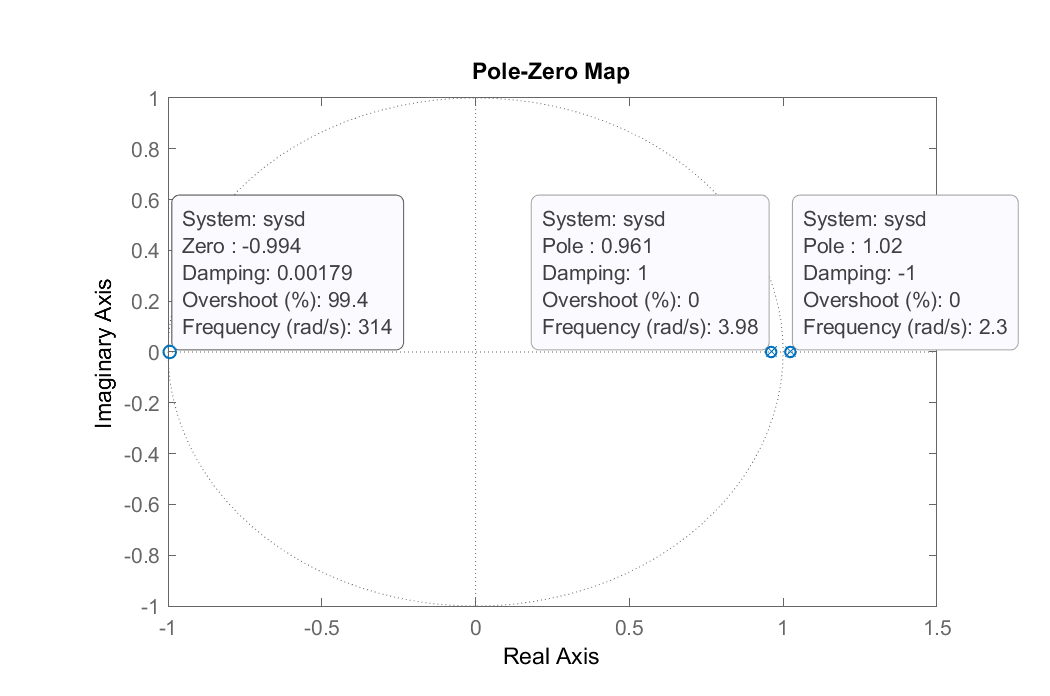
\includegraphics[scale=0.7]{ProjControladores/pzmap_discreto.eps}
    \caption{Círculo unitário de pólos e zeros do modelo discretizado.}
    \label{fig:Circulo-Unitario-Discreto}
\end{figure}{}

Ao analisar a Figura (\ref{fig:Circulo-Unitario-Discreto})), identifica-se um zero em $-0.994$ e os autovalores de malha aberta do sistema discreto como
\begin{equation*}
\lambda_{MA} = \begin{bmatrix}
        0.9610 & 1.0232
    \end{bmatrix}
\end{equation*}
sendo que pólo que mais a direita e fora do círculo unitário, confirma a instabilidade do sistema, de acordo com a literatura. Sendo assim, o controlador deverá levar este pólo para dentro do círculo unitário, ou seja, para dentro da região de estabilidade.

Utilizando-se da função $dlqr$ do $MATLAB$, o ganho $K_{lqr}$ do controlador é encontrado. A utilização deste comando depende das matrizes do espaço de estados do sistema discretizado pelo período de amostragem $T_s$ = $0.01 s$ escolhido - $A$, $B$, $C$ e $D$ - e dos pesos das matrizes da função de custo - $R$ e $Q$. A obtenção dos pólos de malha fechada desejados é obtido ao calcular o ganho do controlador com a função $dlqr$ ou fazendo $(A-BK_{lqr})$. Em relação aos pesos das matrizes da função de custo, definiu-se pesos unitários de modo a conseguir um controlador ótimo entre o custo sobre a ação e a precisão de controle. Abaixo em (\ref{eq:VetorGanhoLQR}) e (\ref{eq:AutovaloresSistemaRealimentadoLQR}), é o mostrado o vetor de ganho $K_{lqr}$ do controlador e o vetor dos pólos de malha fechada $\lambda_{MF}$.
\begin{equation}\label{eq:VetorGanhoLQR}
K_{lqr} = 
        \begin{bmatrix}
            k_{\theta} & k_{\dot{\theta}}
        \end{bmatrix} =
        \begin{bmatrix}
            3.2023 & 1.1508
        \end{bmatrix}
\end{equation}\label{eq:AutovaloresSistemaRealimentadoLQR}
\begin{equation}
\lambda_{MF} = \begin{bmatrix}
        0.9855 & 0.9272
    \end{bmatrix}
\end{equation}

Com intuito de visualizar de forma gráfica o comportamento do modelo não linear com o controlador projetado, elaborou-se uma simulação na plataforma $Simulink$ do $MATLAB$. Sabendo-se que a linearização ocorreu em uma região em torno do equilíbrio que é de $\theta$ = $0^\circ$, setou como condições iniciais para o modelo $\theta_0$ = $5^\circ$ e $\dot{\theta}_0$ = $0^\circ/s$. A Figura (\ref{fig:Implementacao-LQR}) mostra o conjunto de blocos necessários para a implementação do regulador no $Simulink$. 
\begin{figure}[H]
    \centering
    \includegraphics[scale=0.7]{ProjControladores/lqr_control.png}
    \caption{Modelo não linear realimentado pelo controlador $LQR$.}
    \label{fig:Implementacao-LQR}
\end{figure}{}

As seguintes Figuras (\ref{fig:RespostaEstados-LQR}) e (\ref{fig:SinalControle-LQR}) são as respostas dos estados e o sinal de controle respectivamente para o sistema realimentado apenas com o regulador e sem um observador de estados.
\begin{figure}[H]
    \centering
    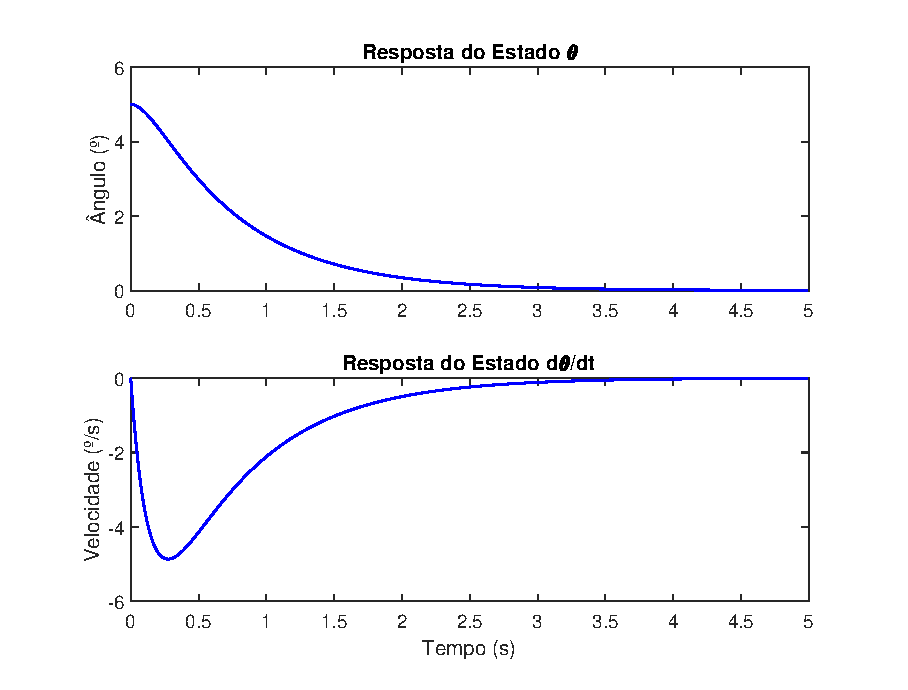
\includegraphics[scale=0.75]{ProjControladores/lqr_estados.eps}
    \caption{Respostas dos estados do sistema para a condição inicial estabelecida.}
    \label{fig:RespostaEstados-LQR}
\end{figure}{}
\begin{figure}[H]
    \centering
    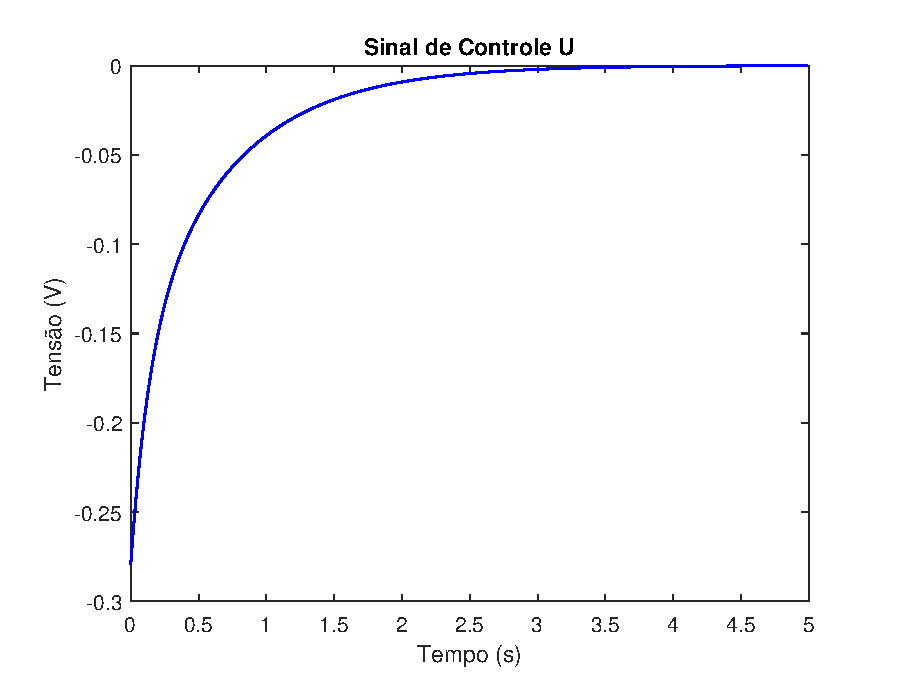
\includegraphics[scale=0.75]{ProjControladores/lqr_sinal_controle.eps}
    \caption{Sinal de controle do sistema para a condição inicial estabelecida.}
    \label{fig:SinalControle-LQR}
\end{figure}{}


\subsection{Estimador de Estados (Filtro de Kalman)}

A subseção (\ref{subsec:ResultadoControladorLQR}) deixa claro que com apenas o ganho do controlador $LQR$, temos um resultado satisfatório. Contudo, o intuito do deste trabalho é realizar o projeto de um estimador de estados para que o mesmo consiga melhorar significativamente o sinal de saída dos mesmos. Quando realizamos a junção tanto do $LQR$ quanto de um estimador de estados, obtemos o $LQG$ que tende a ser mais robusto e menos sensível a ruídos de medição e distúrbios. A simulação do sistema que agora contém um observador de estados, foi realizada sob as mesmas condições da simulação anterior. Sendo assim, as condições iniciais inseridas foram $\theta_0$ = $5^\circ$ e $\dot{\theta}_0$ = $0^\circ/s$. O \textit{design} do sistema com o acréscimo do $LQE$ é visto nas Figuras (\ref{fig:Implementacao-LQG}) e (\ref{fig:Topografia-controladorLQG}).
\begin{figure}[H]
    \centering
    \includegraphics[scale=0.6]{ProjControladores/lqg_control.png}
    \caption{Modelo não linear realimentado pelo controlador $LQG$.}
    \label{fig:Implementacao-LQG}
\end{figure}{}
\begin{figure}[H]
    \centering
    \includegraphics[scale=0.5]{ProjControladores/topografia_lqg.png}
    \caption{Detalhamento do controlador $LQG$.}
    \label{fig:Topografia-controladorLQG}
\end{figure}{}

Com essa nova topografia, realizamos o mesmo teste realizado anteriormente no qual a planta tinha apenas o regulador. As condições iniciais para a planta são as mesmas como já mencionado, o que difere agora são as condições iniciais do observador que foram setadas como sendo $\hat{\theta}$ = $\dot{\hat{\theta}}$ = $0$. Abaixo, nas Figuras (\ref{fig:RespostaEstados-LQG}) e (\ref{fig:SinalControle-LQG}) é visto a resposta dos sinais dos estados e do sinal de controle respectivamente.

\begin{figure}[H]
    \centering
    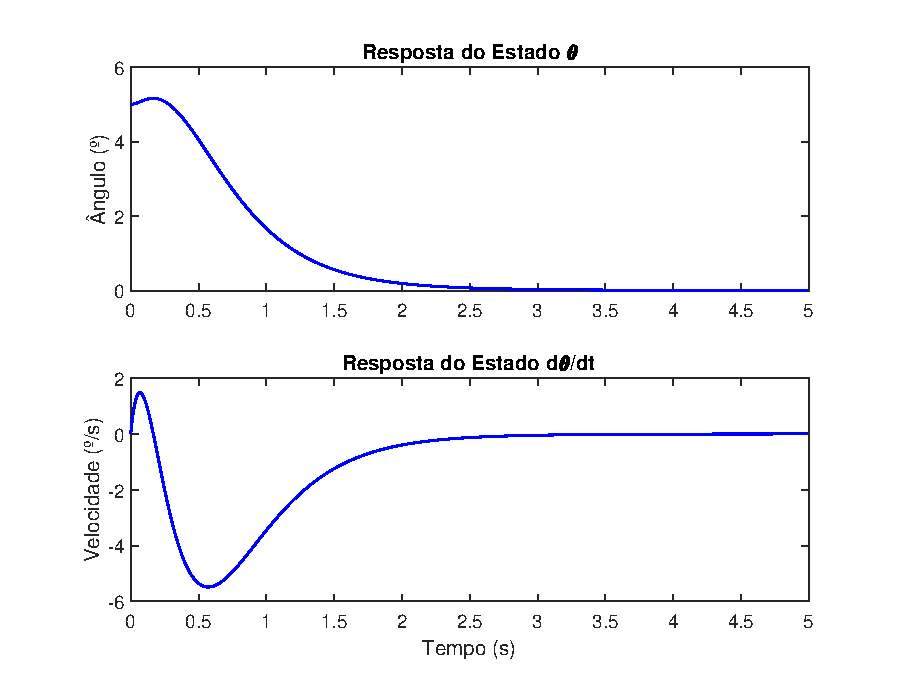
\includegraphics[scale=0.75]{ProjControladores/lqg_estados.eps}
    \caption{Respostas dos estados do sistema para a condição inicial estabelecida.}
    \label{fig:RespostaEstados-LQG}
\end{figure}{}

\begin{figure}[H]
    \centering
    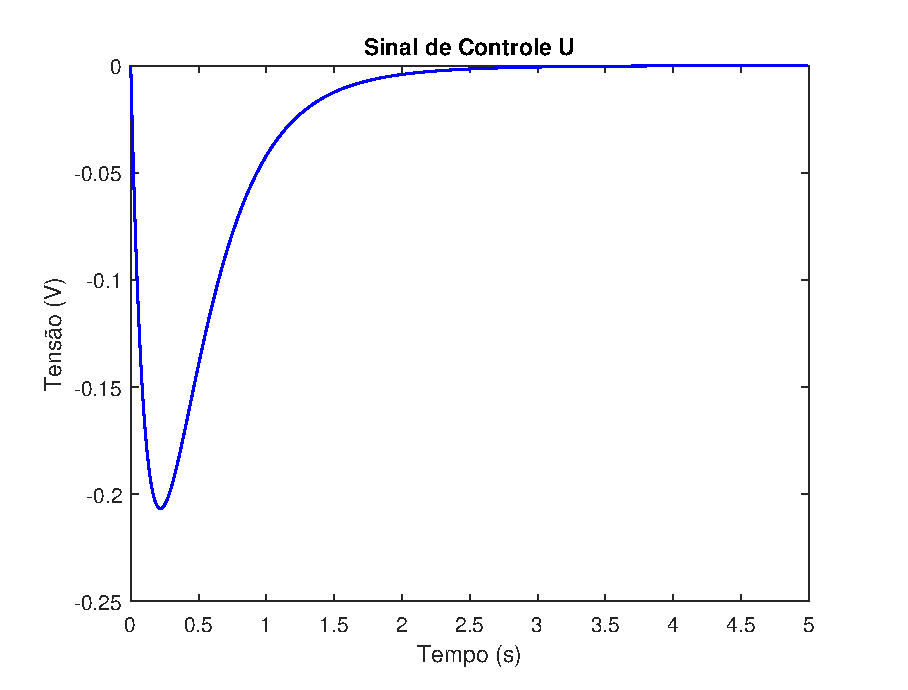
\includegraphics[scale=0.75]{ProjControladores/lqg_sinal_controle.eps}
    \caption{Sinal de controle do sistema para a condição inicial estabelecida.}
    \label{fig:SinalControle-LQG}
\end{figure}{}


\subsubsection{Inserção de Distúrbio e Ruído de Medição ao Sistema}

Como visto, em condições ideais e não reais já que todo sinal de medição haverá algum tipo de ruído, distúrbio e outras perturbações que está sendo até simplificado já no modelo, percebe-se que o controlador atua muito bem e sem dificuldade para estabilizar a planta. Dessa maneira, para testar o modelo de forma mais real e obter um resultado mais fidedigno do que realmente irá acontecer ao embarcar o controlador na planta física, resolveu-se incorporar ao sistema um sinal de ruído branco na resposta do sensor. Esse sinal, como visto na Figura (\ref{fig:SinalRuidoBranco}), possui um \textit{range} $\pm 1^\circ$, ou seja, quer dizer o sensor pode estar errando tanto $1^\circ$ positivo quanto $1^\circ$ negativo.
\begin{figure}[H]
    \centering
    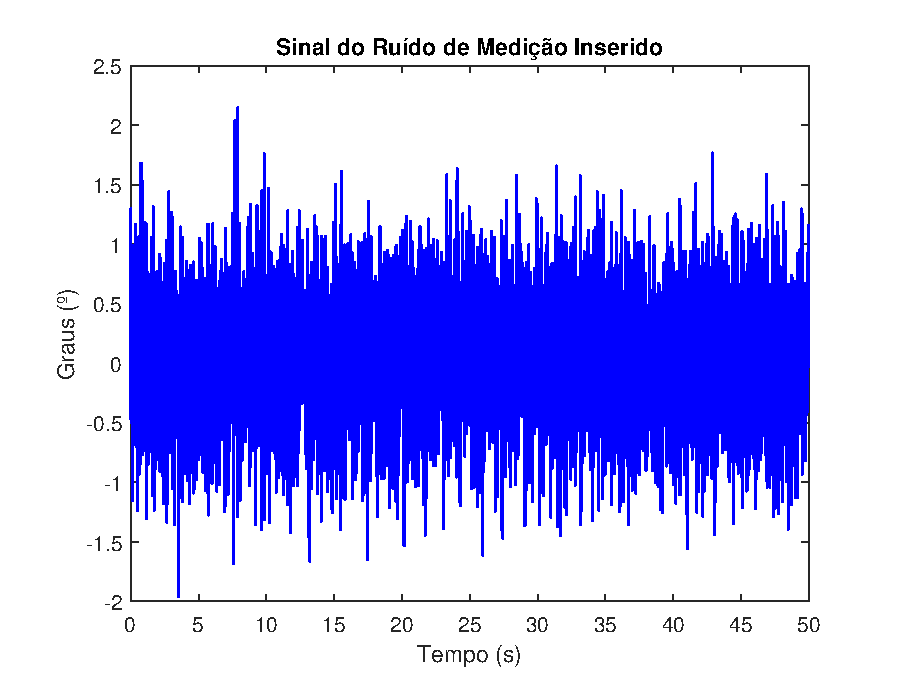
\includegraphics[scale=0.75]{ProjControladores/ruido_branco_medicao.eps}
    \caption{Sinal do ruído branco de medição.}
    \label{fig:SinalRuidoBranco}
\end{figure}{}

Além do ruído inserido, também decidiu-se por aplicar um distúrbio na simulação com intuito de visualizar o comportamento do controlador perante a uma adversidade, uma vez que após um certo tempo de início o sistema tende a ficar estável. Sendo assim, de forma proposital aplicou um sinal quadrático de duração de 0.5$s$, iniciando em t = 20$s$ e com amplitude de $3^\circ$. O \textit{design} do sistema com essas novas dificuldades impostas ao controlador é visto na Figura (\ref{fig:Implementacao-LQG-real}).
\begin{figure}[H]
    \centering
    \includegraphics[scale=0.5]{ProjControladores/lqg_control_real.png}
    \caption{Modelo não linear realimentado pelo controlador $LQG$ com inserção de distúrbio e ruídos.}
    \label{fig:Implementacao-LQG-real}
\end{figure}{}

A Figura (\ref{fig:Topografia-controladorLQG-real}) mostra o detalhamento do controlador $LQG$ com o distúrbio e o ruído aplicado. Como é visto, o sinal do sinal do distúrbio é somado juntamente ao estado $\hat{\theta}$, antes de passar pelo regulador. Por sua vez, o sinal de ruído é somado ao sinal de medição realimentado.
\begin{figure}[H]
    \centering
    \includegraphics[scale=0.5]{ProjControladores/topografia_lqg_real.png}
    \caption{Detalhamento do controlador $LQG$ com a inserção de distúrbio e ruído de medição.}
    \label{fig:Topografia-controladorLQG-real}
\end{figure}{}

Contudo, para aproximar mais da realidade é inserido ao sistema um sinal quadrático de duração de 0.5$s$, iniciando em t = 20$s$ e com amplitude de $3^\circ$.

\begin{figure}[H]
    \centering
    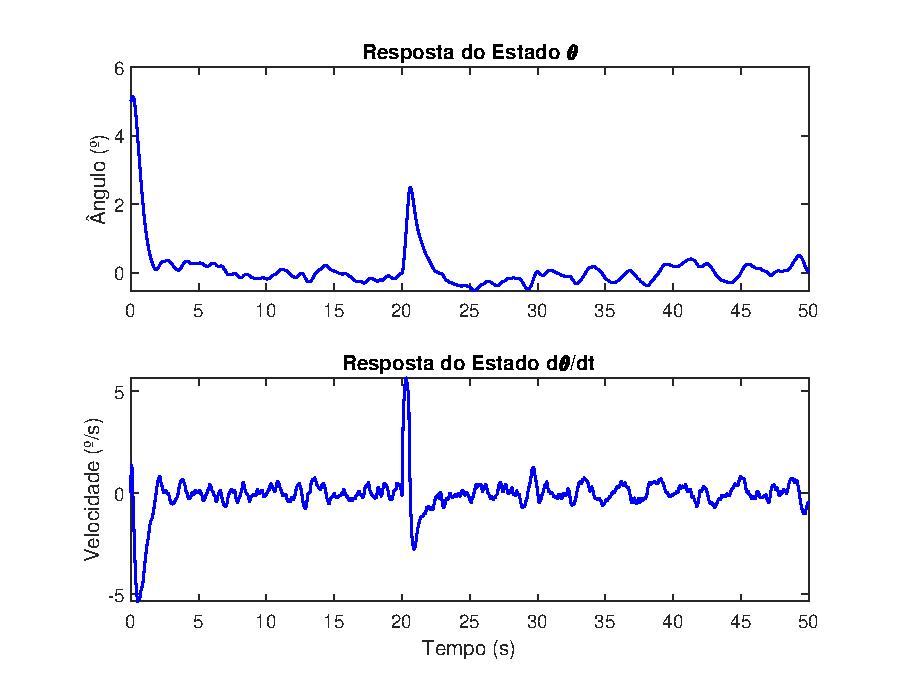
\includegraphics[scale=0.75]{ProjControladores/lqg_real_estados.eps}
    \caption{Respostas dos estados do sistema para a condição inicial estabelecida.}
    \label{fig:RespostaEstados-LQG-real}
\end{figure}{}

\begin{figure}[H]
    \centering
    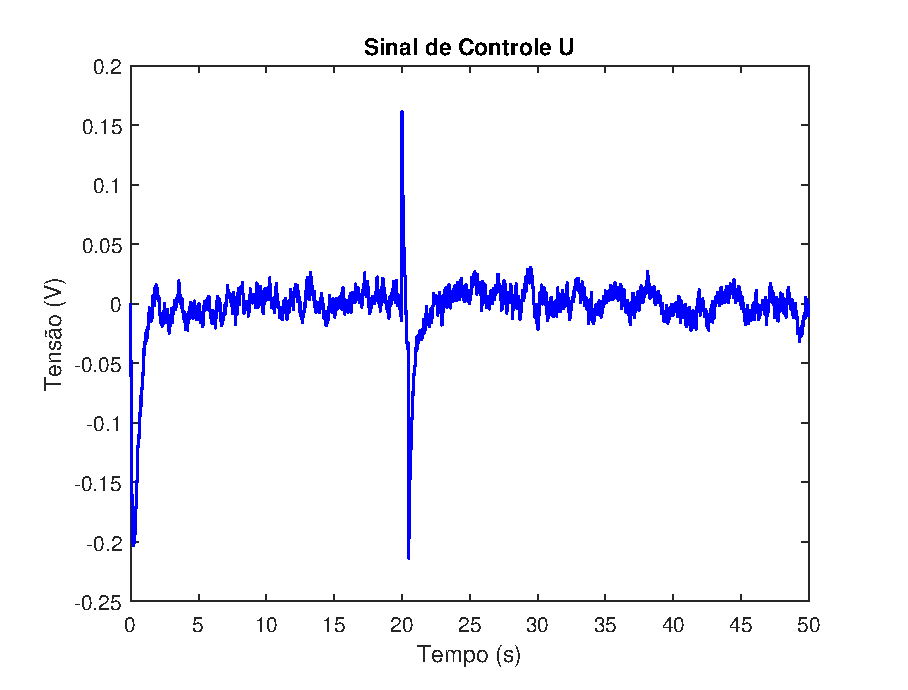
\includegraphics[scale=0.75]{ProjControladores/lqg_real_sinal_controle.eps}
    \caption{Sinal de controle do sistema para a condição inicial estabelecida.}
    \label{fig:SinalControle-LQG-real}
\end{figure}{}



